\providecommand{\main}{../../../..}
\documentclass[\main/dresen_thesis.tex]{subfiles}
\begin{document}
  \label{sec:looselyPackedNS:layers:pnr}
  \begin{figure}[tb]
    \centering
    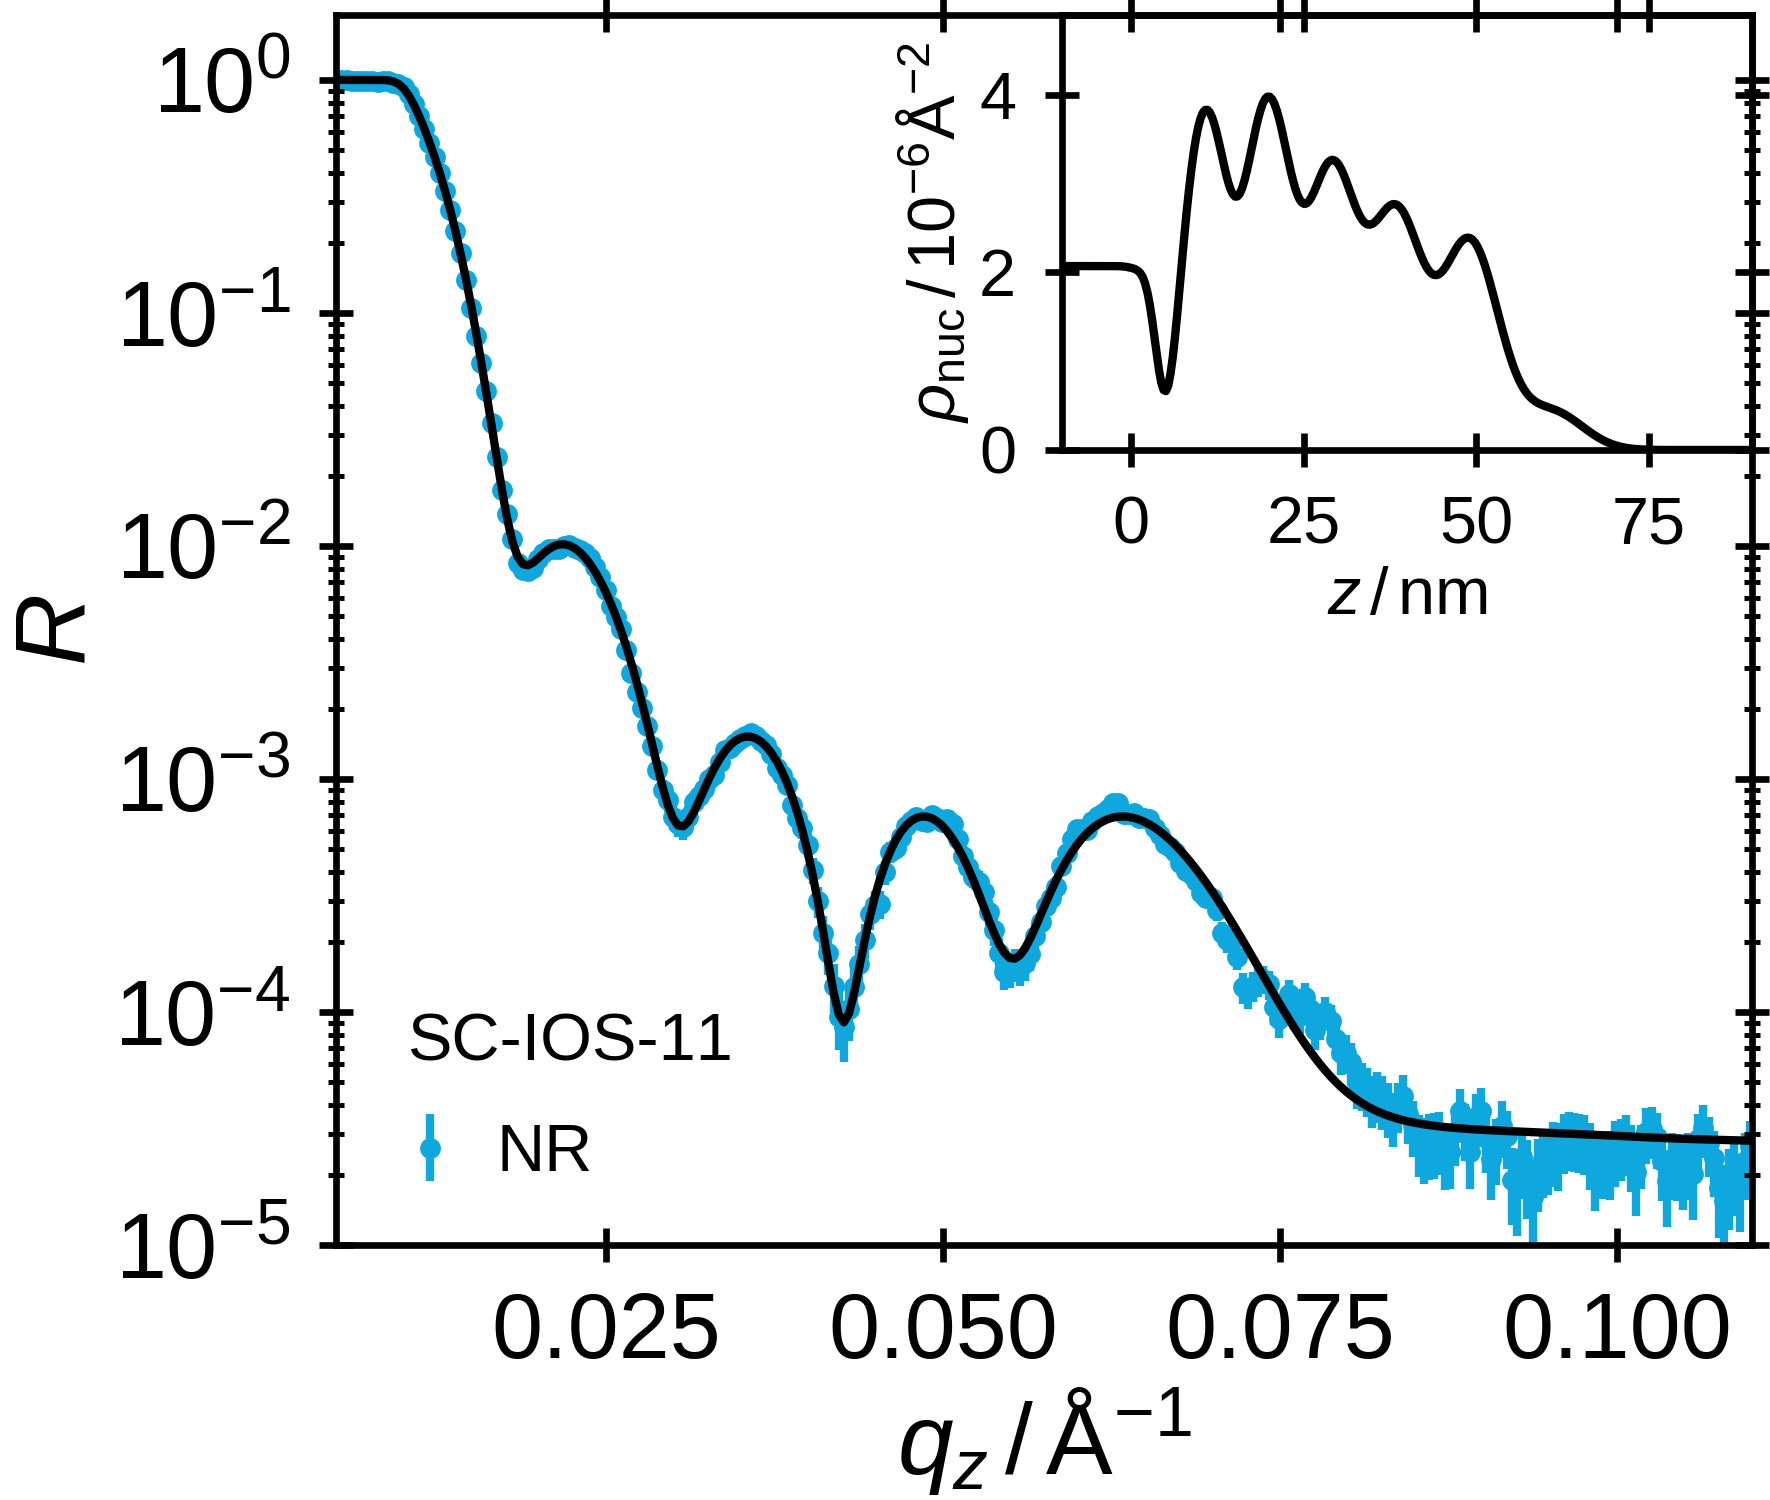
\includegraphics{looselyPackedNP_VerticalStructure_SC-IOS-11_PNR}
    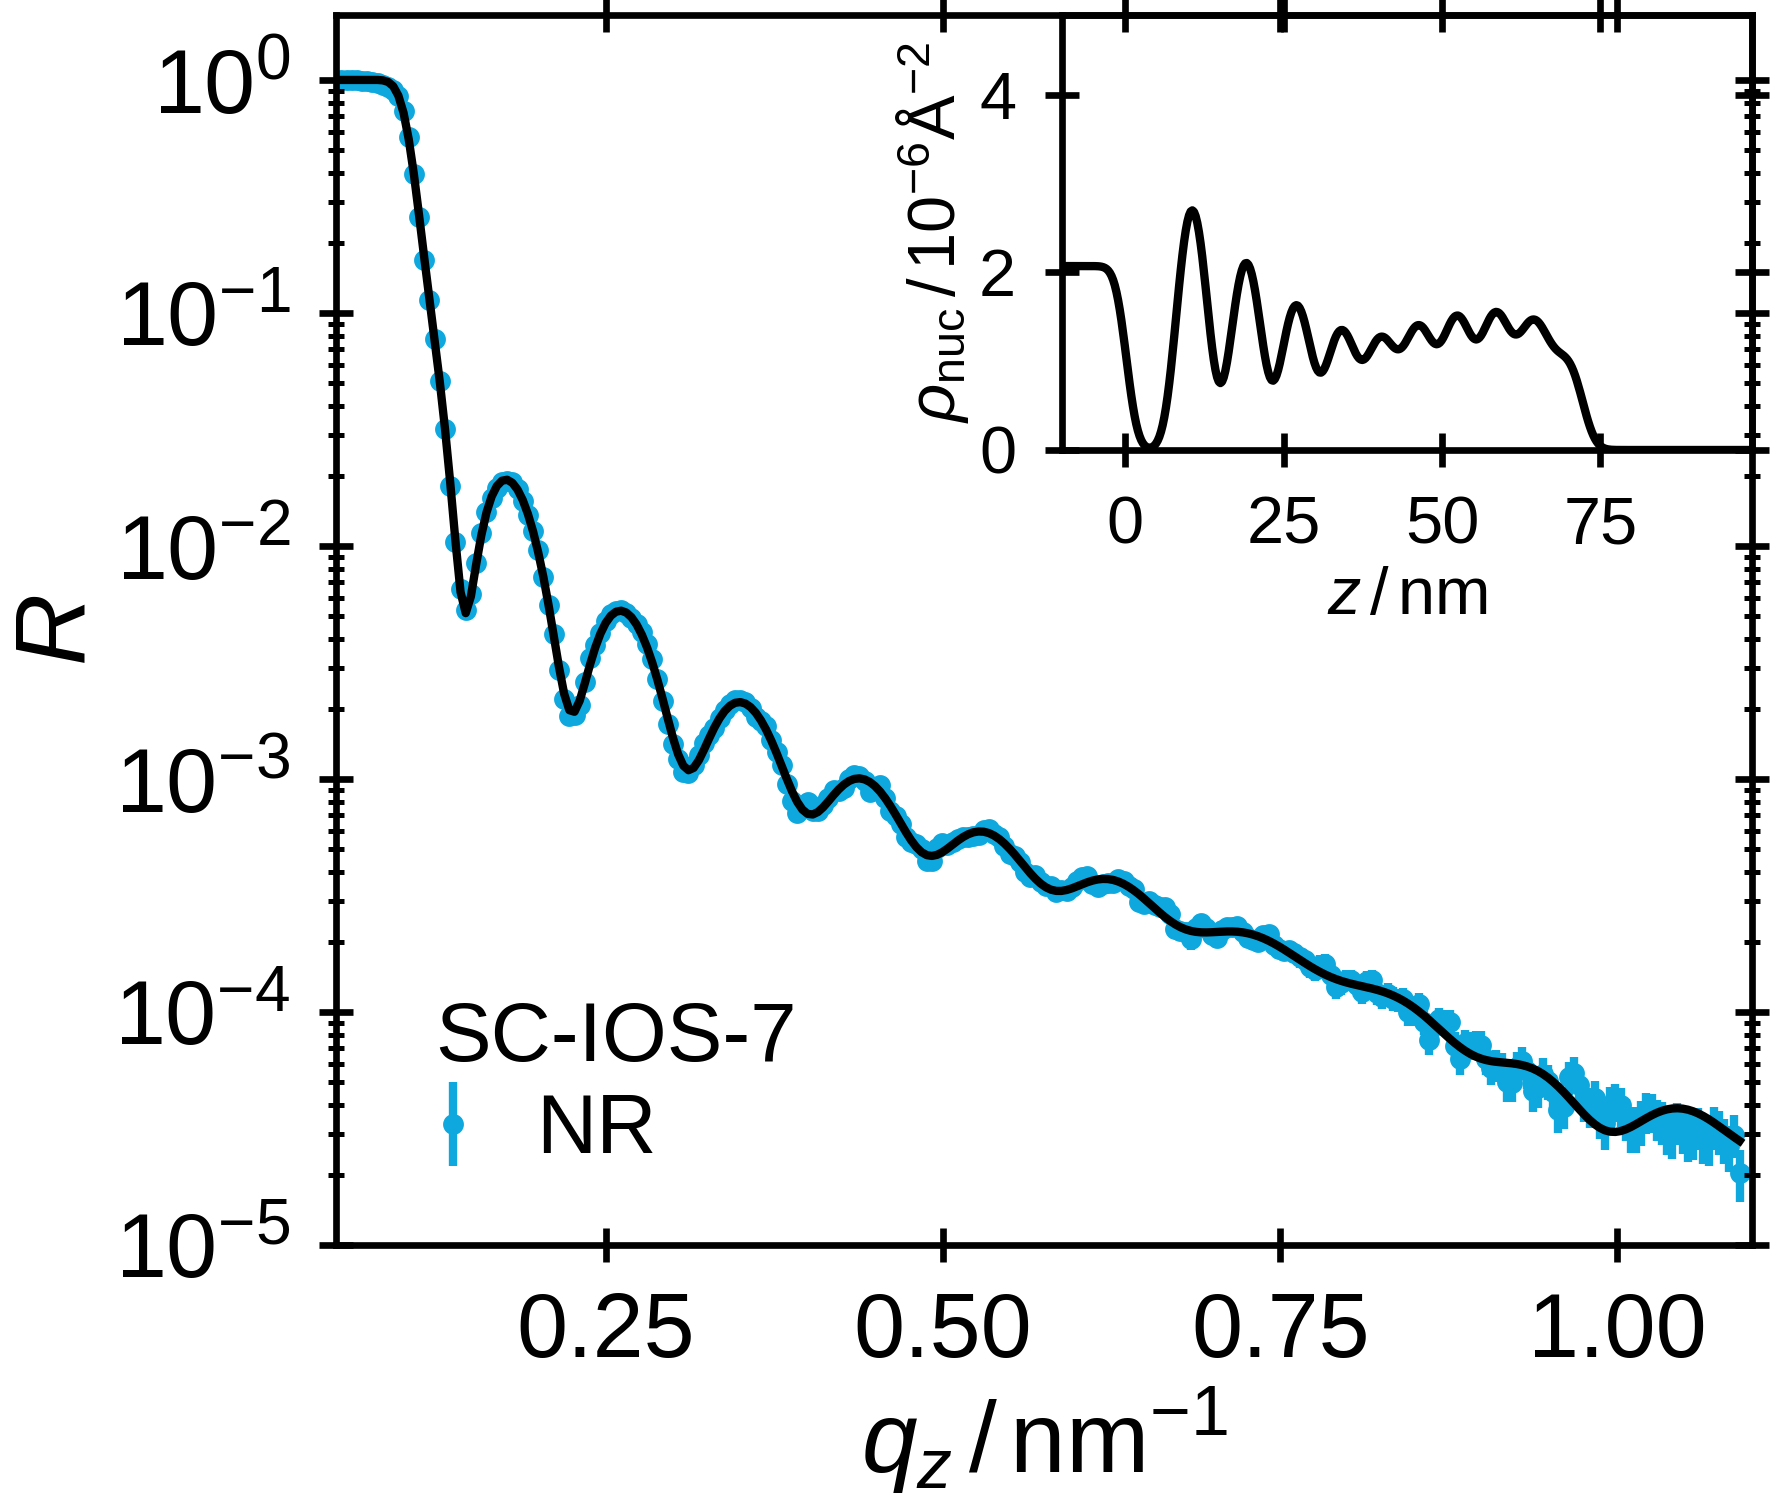
\includegraphics{looselyPackedNP_VerticalStructure_SC-IOS-7_PNR}
    \caption{\label{fig:looselyPackedNP:layer:xrr}X-ray reflectometry from SC-IOS-11 (left) and SC-IOS-7 (right). The inset shows the scattering length density model of the fitted reflectometry curve (black).}
  \end{figure}
  % \begin{table}[!htbp]
  %   \centering
  %   \caption{\label{tab:looselyPackedNP:nanoparticle:gisaxs}Parameters for the hard-sphere structure factor in Percus-Yervick approximation shown in \reffig{fig:looselyPackedNP:layer:gisaxs} for both SC-IOS-11 and SC-IOS-7. $R_\mathrm{HS}$ is the hard-sphere radius and $\eta$ the packing fraction of the structure factor.}
  %   \begin{tabular}{ c | l | l }
  %     \rule{0pt}{2ex} \textbf{GISAXS}  & \textbf{SC-IOS-11} & \textbf{SC-IOS-7} \\
  %     \hline
  %     \rule{0pt}{2ex} $R_\mathrm{HS} \, / \unit{nm}$          & $5.655(2)$           & $3.872(4)$\\
  %     \rule{0pt}{2ex} $\eta          \, / \unit{\%}$          & $43.88(3)$           & $34.20(9)$\\
  %     \hline
  %   \end{tabular}
  % \end{table}


  % \begin{figure}[tb]
  %   \centering
  %   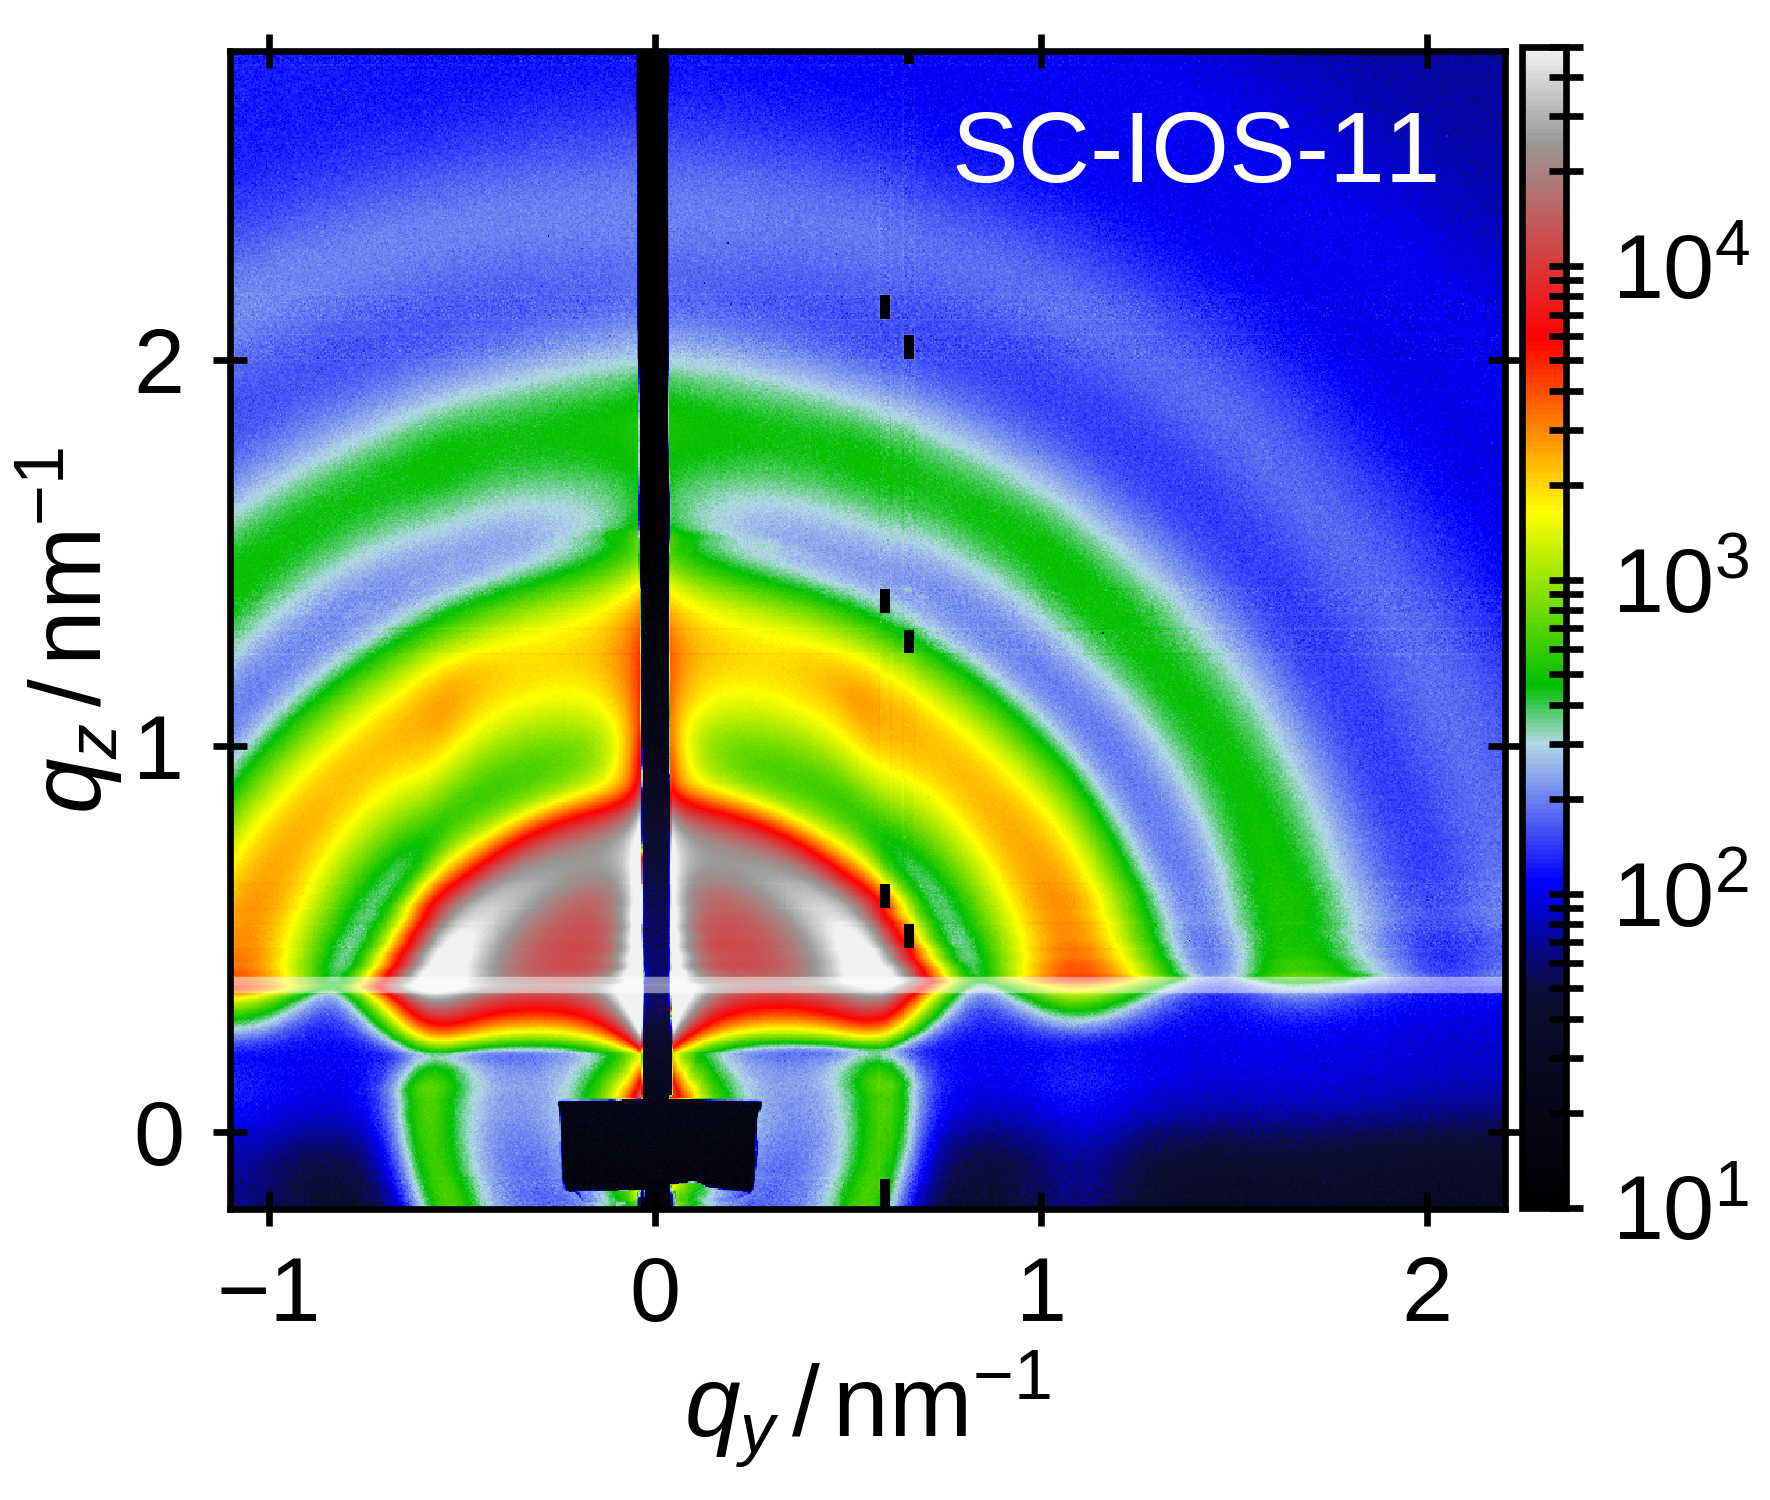
\includegraphics{looselyPackedNP_GISAXS_SC-IOS-11}
  %   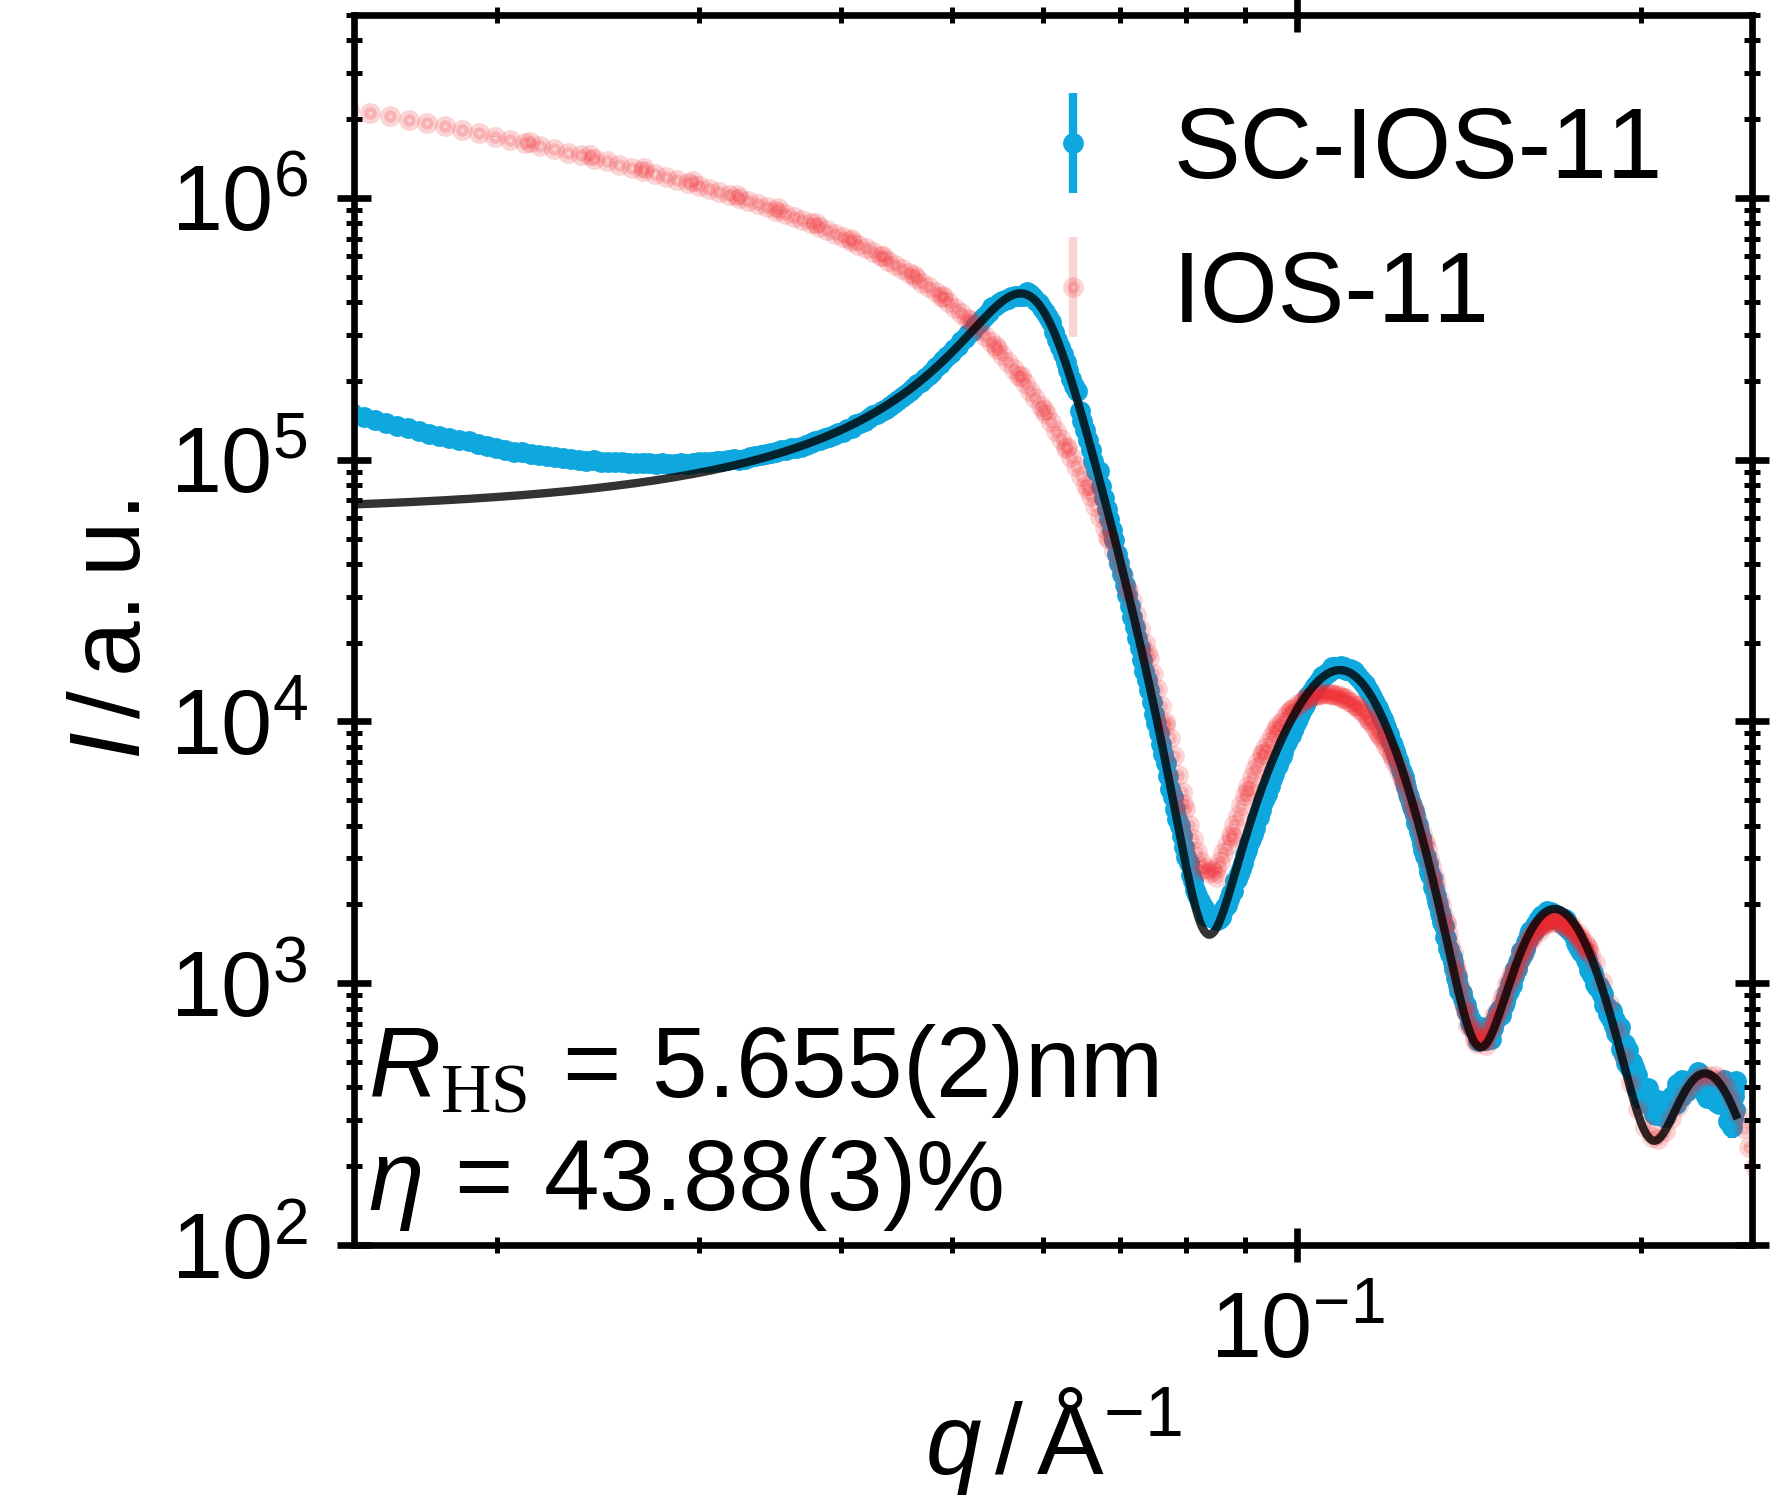
\includegraphics{looselyPackedNP_GISAXS_StructureFactor_SC-IOS-11}
  %   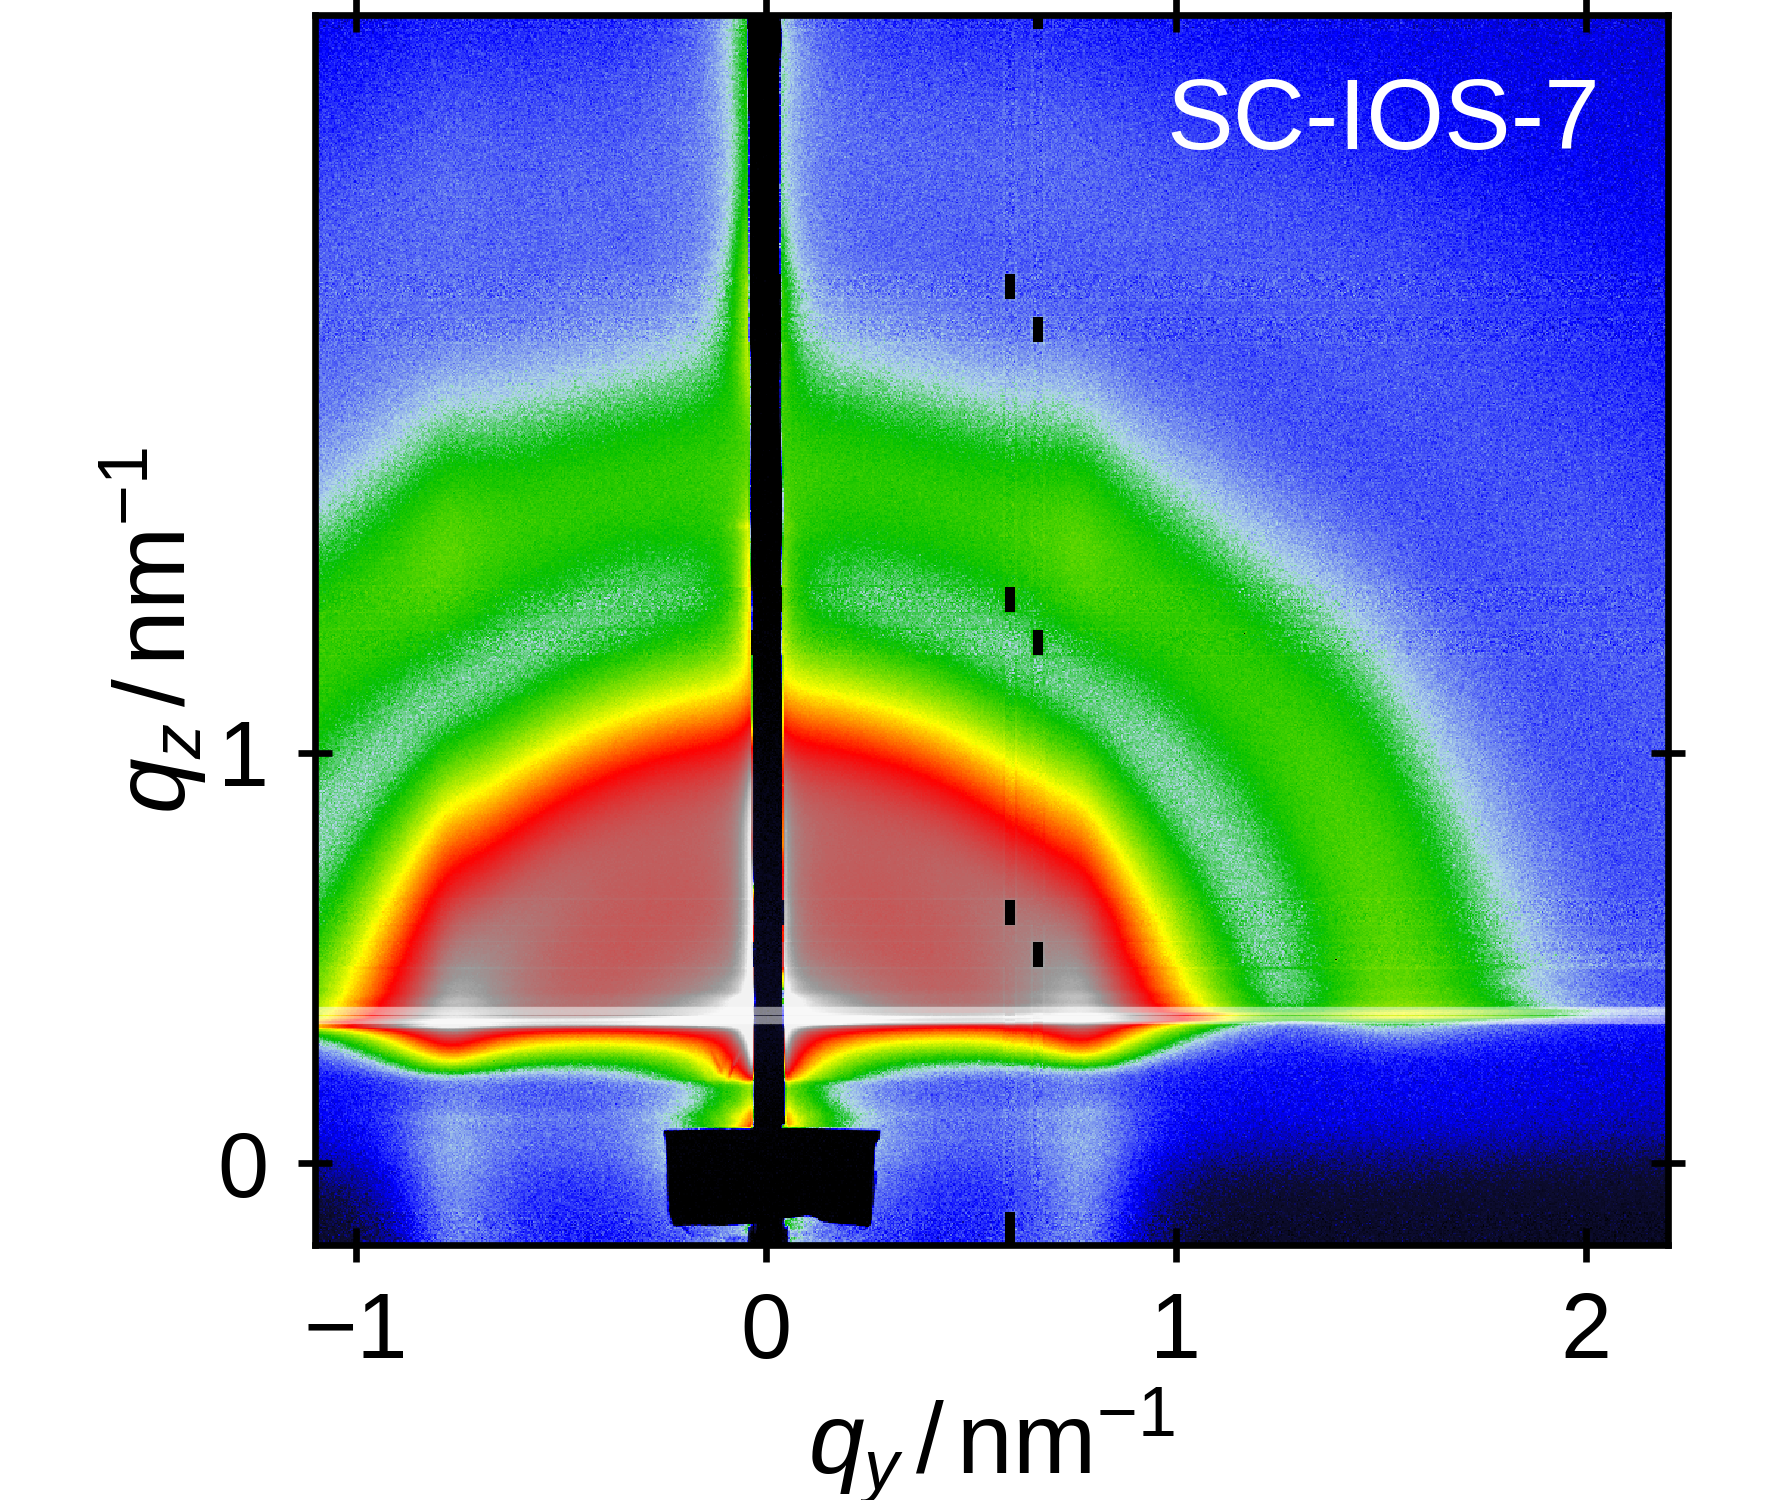
\includegraphics{looselyPackedNP_GISAXS_SC-IOS-7}
  %   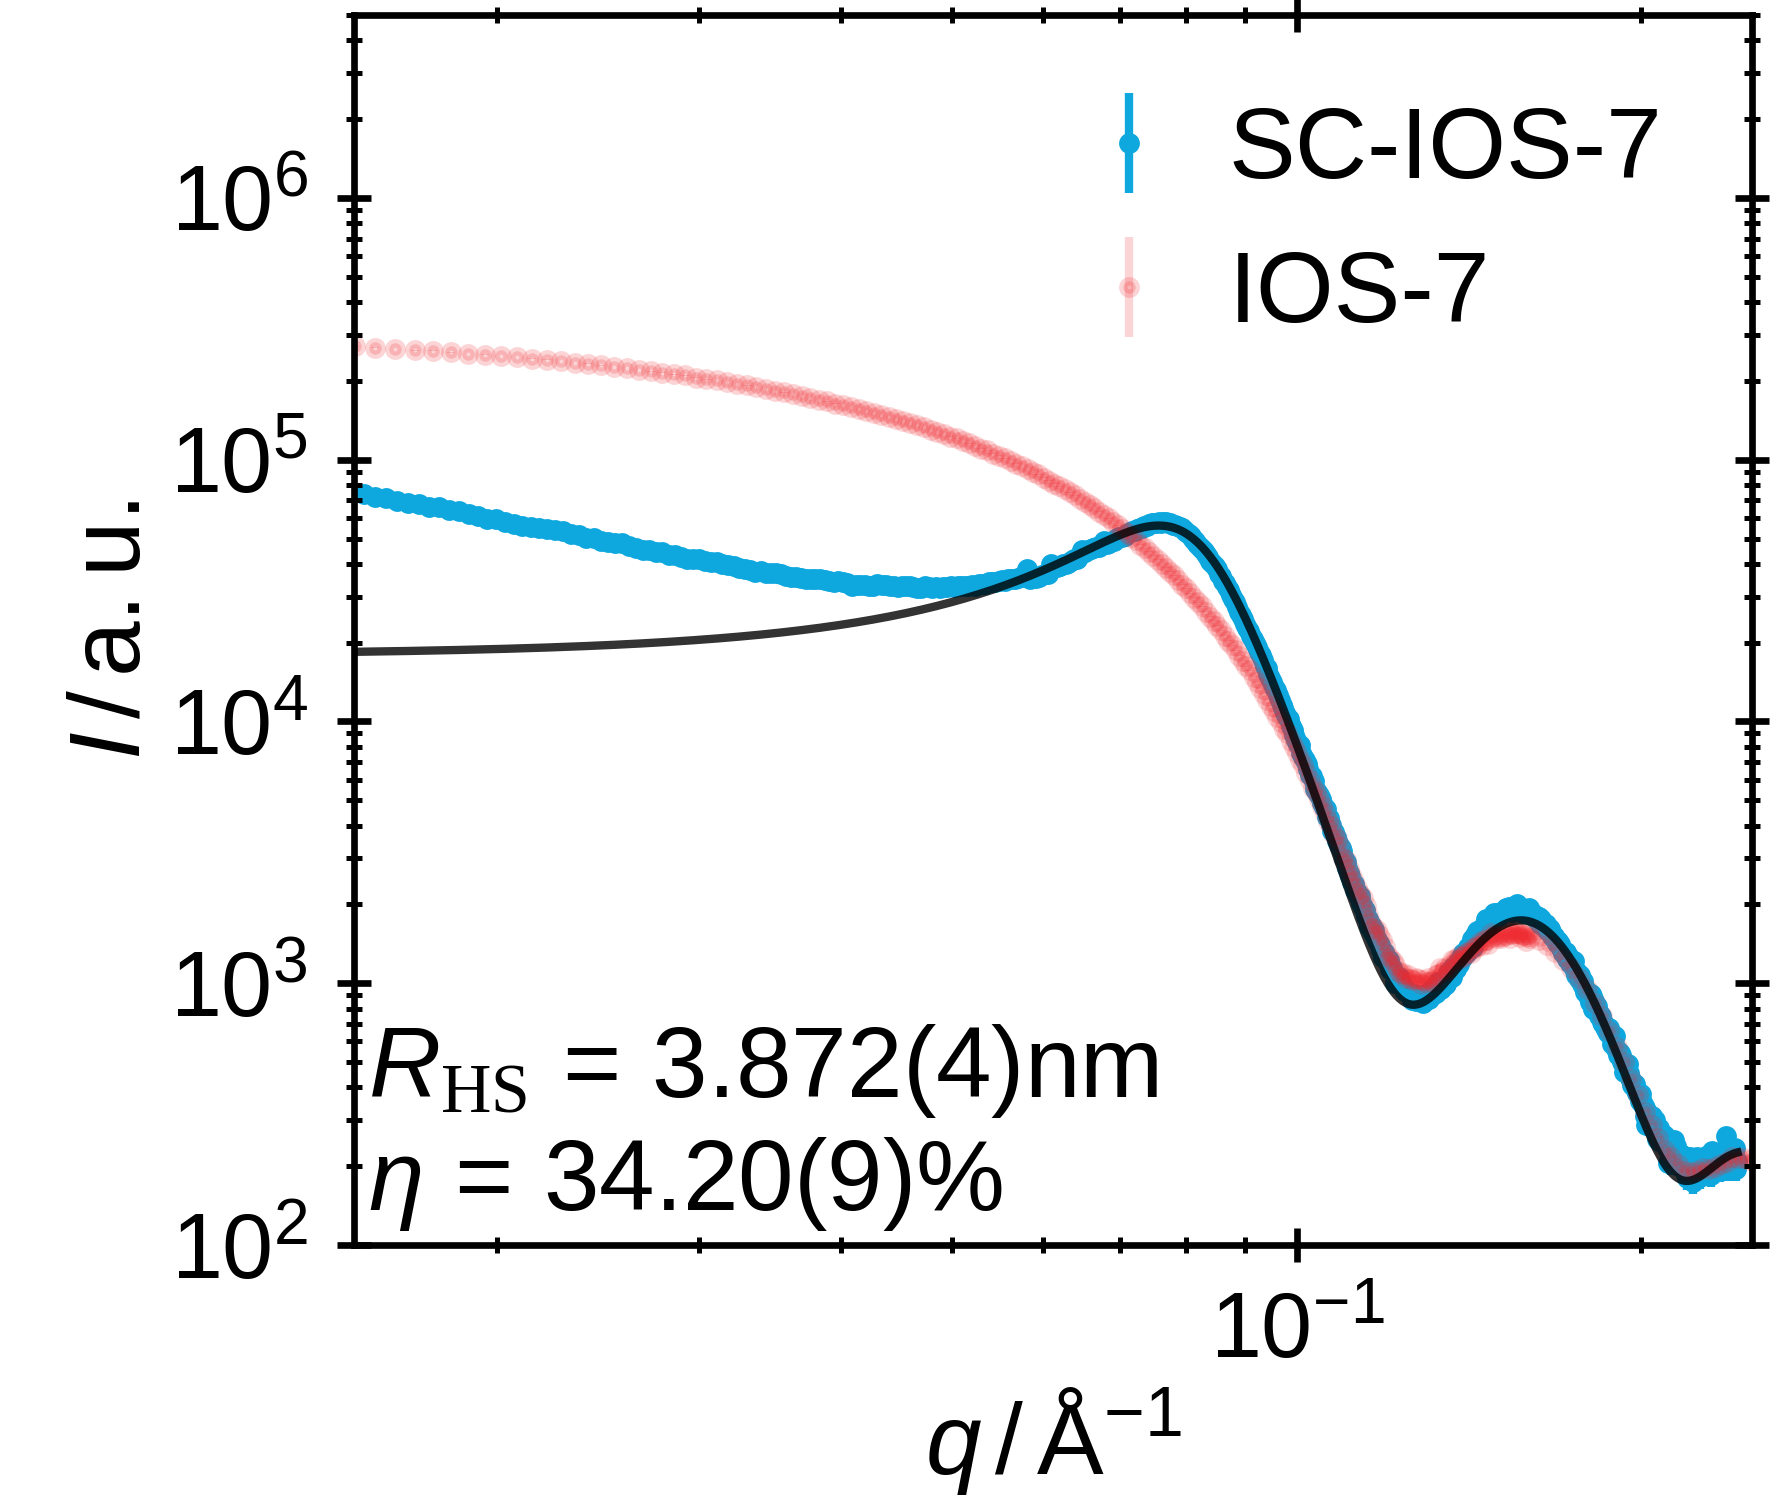
\includegraphics{looselyPackedNP_GISAXS_StructureFactor_SC-IOS-7.png}
  %   \caption{\label{fig:looselyPackedNP:layer:gisaxs}GISAXS detector images (left) of IOS-11 (upper) and IOS-7 (lower) measured at the BM26B beam line at the ESRF under an incident angle of $\alpha_i \eq 0.2 \unit{^\circ}$. The  integrated data in the Yoneda band (right, blue curve), marked by the white stripe on the detector images, is fitted to the hard-sphere structure factor in Percus-Yervick approximation, with parameters listed in \reftab{tab:looselyPackedNP:nanoparticle:gisaxs}. The SAXS form factor of the nanoparticles in dispersion is shown for comparison (red curve). The black area around $q_y \eq 0 \unit{nm^{-1}}$ is the beam stop, whereas the small black rectangles in the detector images are gaps due to inactive areas of the detector. }
  % \end{figure}

  \begin{table}[!htbp]
    \centering
    \caption{\label{tab:looselyPackedNP:nanoparticle:xrr}Parameters for the layer of multiple nanospheres shown in \reffig{fig:looselyPackedNP:layer:xrr}. The parameters $\eta$ are the two dimensional packing density for each layer and $\Delta z$ are the shifts of the layer center from the pitch $\sqrt{8/3} (R+D_\mathrm{OA}$). The other parameters are the thickness of the spacer layer on the substrate $d_\mathrm{spacer}$, its SLD $\rho_\mathrm{spacer}$, the substrate roughness $\sigma$, the rate of roughness increase with layer height $\Delta \sigma$, and the wavelength spread of the instrument $\sigma_\lambda / \lambda$. The nanosphere parameters are fixed from SAXS.}
    \begin{tabular}{ c | l | l }
      \rule{0pt}{2ex} \textbf{XRR}  & \textbf{SC-IOS-11} & \textbf{SC-IOS-7} \\
      \hline
       $\eta_1     \, / \unit{\%}$                                  & $50.9(4)$         & $34(1)$    \\
       $\eta_2     \, / \unit{\%}$                                  & $55.4(4)$         & $32(1)$    \\
       $\eta_3     \, / \unit{\%}$                                  & $52.9(5)$         & $30(2)$    \\
       $\eta_4     \, / \unit{\%}$                                  & $49.8(6)$         & $33(3)$    \\
       $\eta_5     \, / \unit{\%}$                                  & $53.4(8)$         & $38(3)$    \\
       $\eta_6     \, / \unit{\%}$                                  & $28.6(1.0)$       & $40(3)$    \\
       $\eta_7     \, / \unit{\%}$                                  &                   & $41(3)$    \\
       $\eta_8     \, / \unit{\%}$                                  &                   & $44(3)$    \\
       $\eta_9     \, / \unit{\%}$                                  &                   & $43(7)$    \\
       $\eta_{10}     \, / \unit{\%}$                               &                   & $34(9)$    \\
       $\eta_{11}     \, / \unit{\%}$                               &                   & $8(10)$    \\
       \hline
       $\Delta z_1 \, / \unit{nm} $                                 & $-1.04(3)$        & $-1.33(6)$ \\
       $\Delta z_2 \, / \unit{nm} $                                 & $-2.60(3)$        & $-1.33(7)$ \\
       $\Delta z_3 \, / \unit{nm} $                                 & $-2.68(3)$        & $-1.13(8)$ \\
       $\Delta z_4 \, / \unit{nm} $                                 & $-2.95(4)$        & $-1.22(6)$ \\
       $\Delta z_5 \, / \unit{nm} $                                 & $-2.67(4)$        & $-1.40(6)$ \\
       $\Delta z_6 \, / \unit{nm} $                                 & $-1.82(10)$       & $-1.46(7)$ \\
       $\Delta z_7 \, / \unit{nm} $                                 &                   & $-1.41(9)$ \\
       $\Delta z_8 \, / \unit{nm} $                                 &                   & $-1.2(1)$   \\
       $\Delta z_9 \, / \unit{nm} $                                 &                   & $-0.4(5)$    \\
       $\Delta z_{10} \, / \unit{nm} $                              &                   & $-2.4(8)$   \\
       $\Delta z_{11} \, / \unit{nm} $                              &                   & $-1.5(19)$  \\
       \hline
       $d_\mathrm{spacer}   \, / \unit{nm} $                        & $5.15(3)$         & $5.27(2)$  \\
       $\rho_\mathrm{spacer}\, / \unit{10^{-6} \angstrom^{-2}} $    & $11.9(2)$         & $2.2(1)$ \\
       $\sigma     \, / \unit{nm} $                                 & $0.65(1)$         & $0.70(1)$  \\
       $\Delta \sigma$                                              & $0.034(1)$        & $0.036(1)$ \\
       $\sigma_\lambda / \lambda\, / \unit{\%}$                     & \multicolumn{2}{c}{$1.1(2)$} \\
      \hline
       $R             \, / \unit{nm}$                               & $5.41$         & $3.54$ \\
       $D_\mathrm{OA} \, / \unit{nm}$                               & $1.82$         & $1.69$ \\
       $\sigma_R      \, / \unit{\%}$                               & $5.45$         & $7.52$ \\
       $\rho_\mathrm{core}\, / \unit{10^{-6} \angstrom^{-2}}      $ & \multicolumn{2}{c}{$40.5$}\\
       $\rho_\mathrm{shell}\, / \unit{10^{-6} \angstrom^{-2}}     $ & \multicolumn{2}{c}{$8.52$}\\
       $\rho_\mathrm{substrate}\, / \unit{10^{-6} \angstrom^{-2}} $ & \multicolumn{2}{c}{$20.1$}\\
      \hline
    \end{tabular}
  \end{table}
  \begin{figure}[tb]
    \centering
    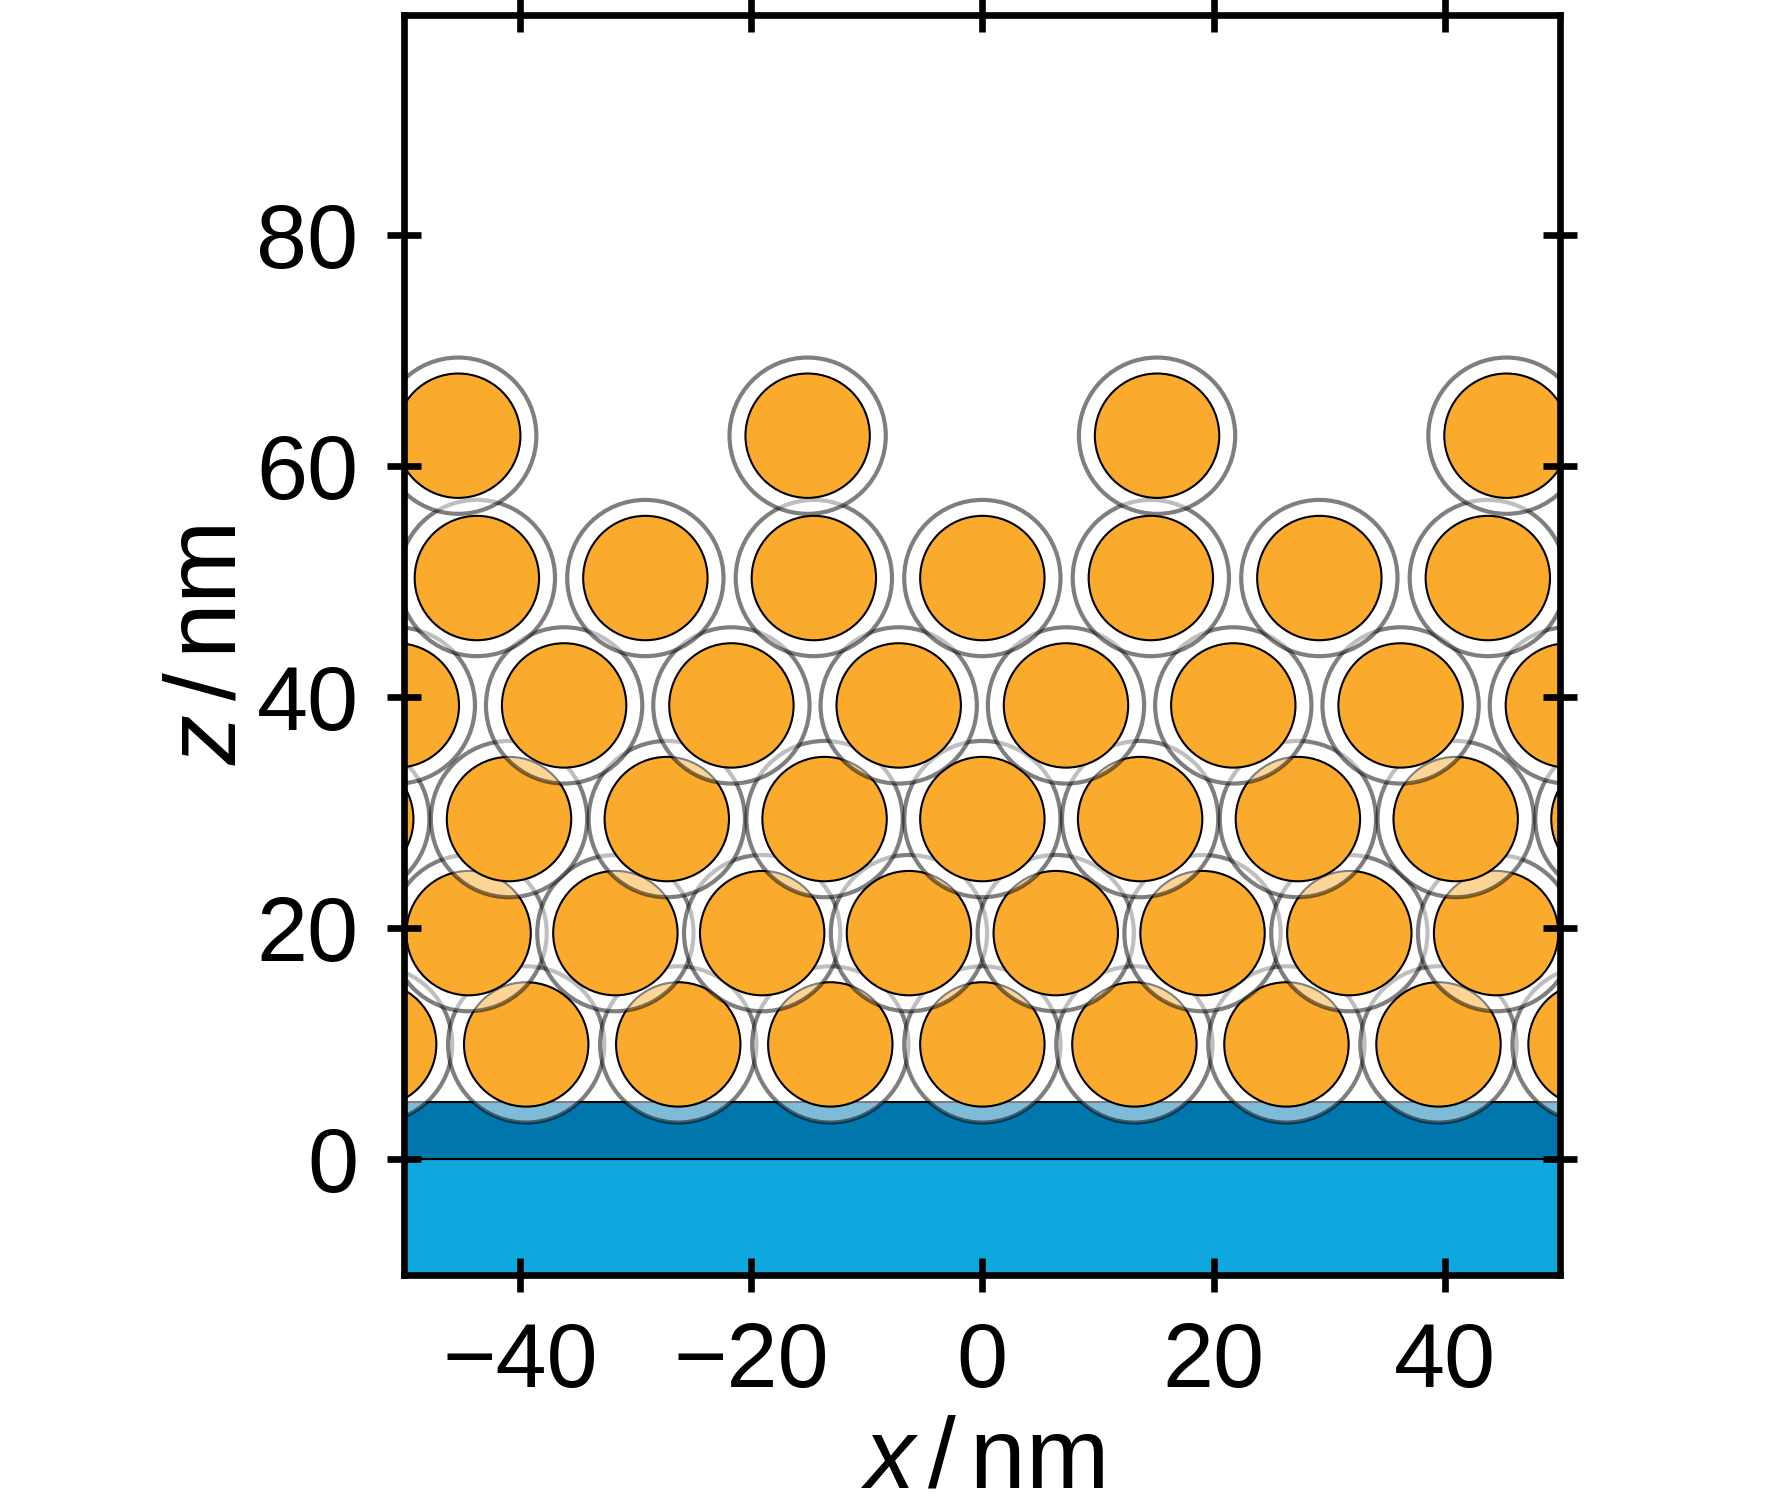
\includegraphics{looselyPackedNP_VerticalStructure_SC-IOS-11_PNRDepiction}
    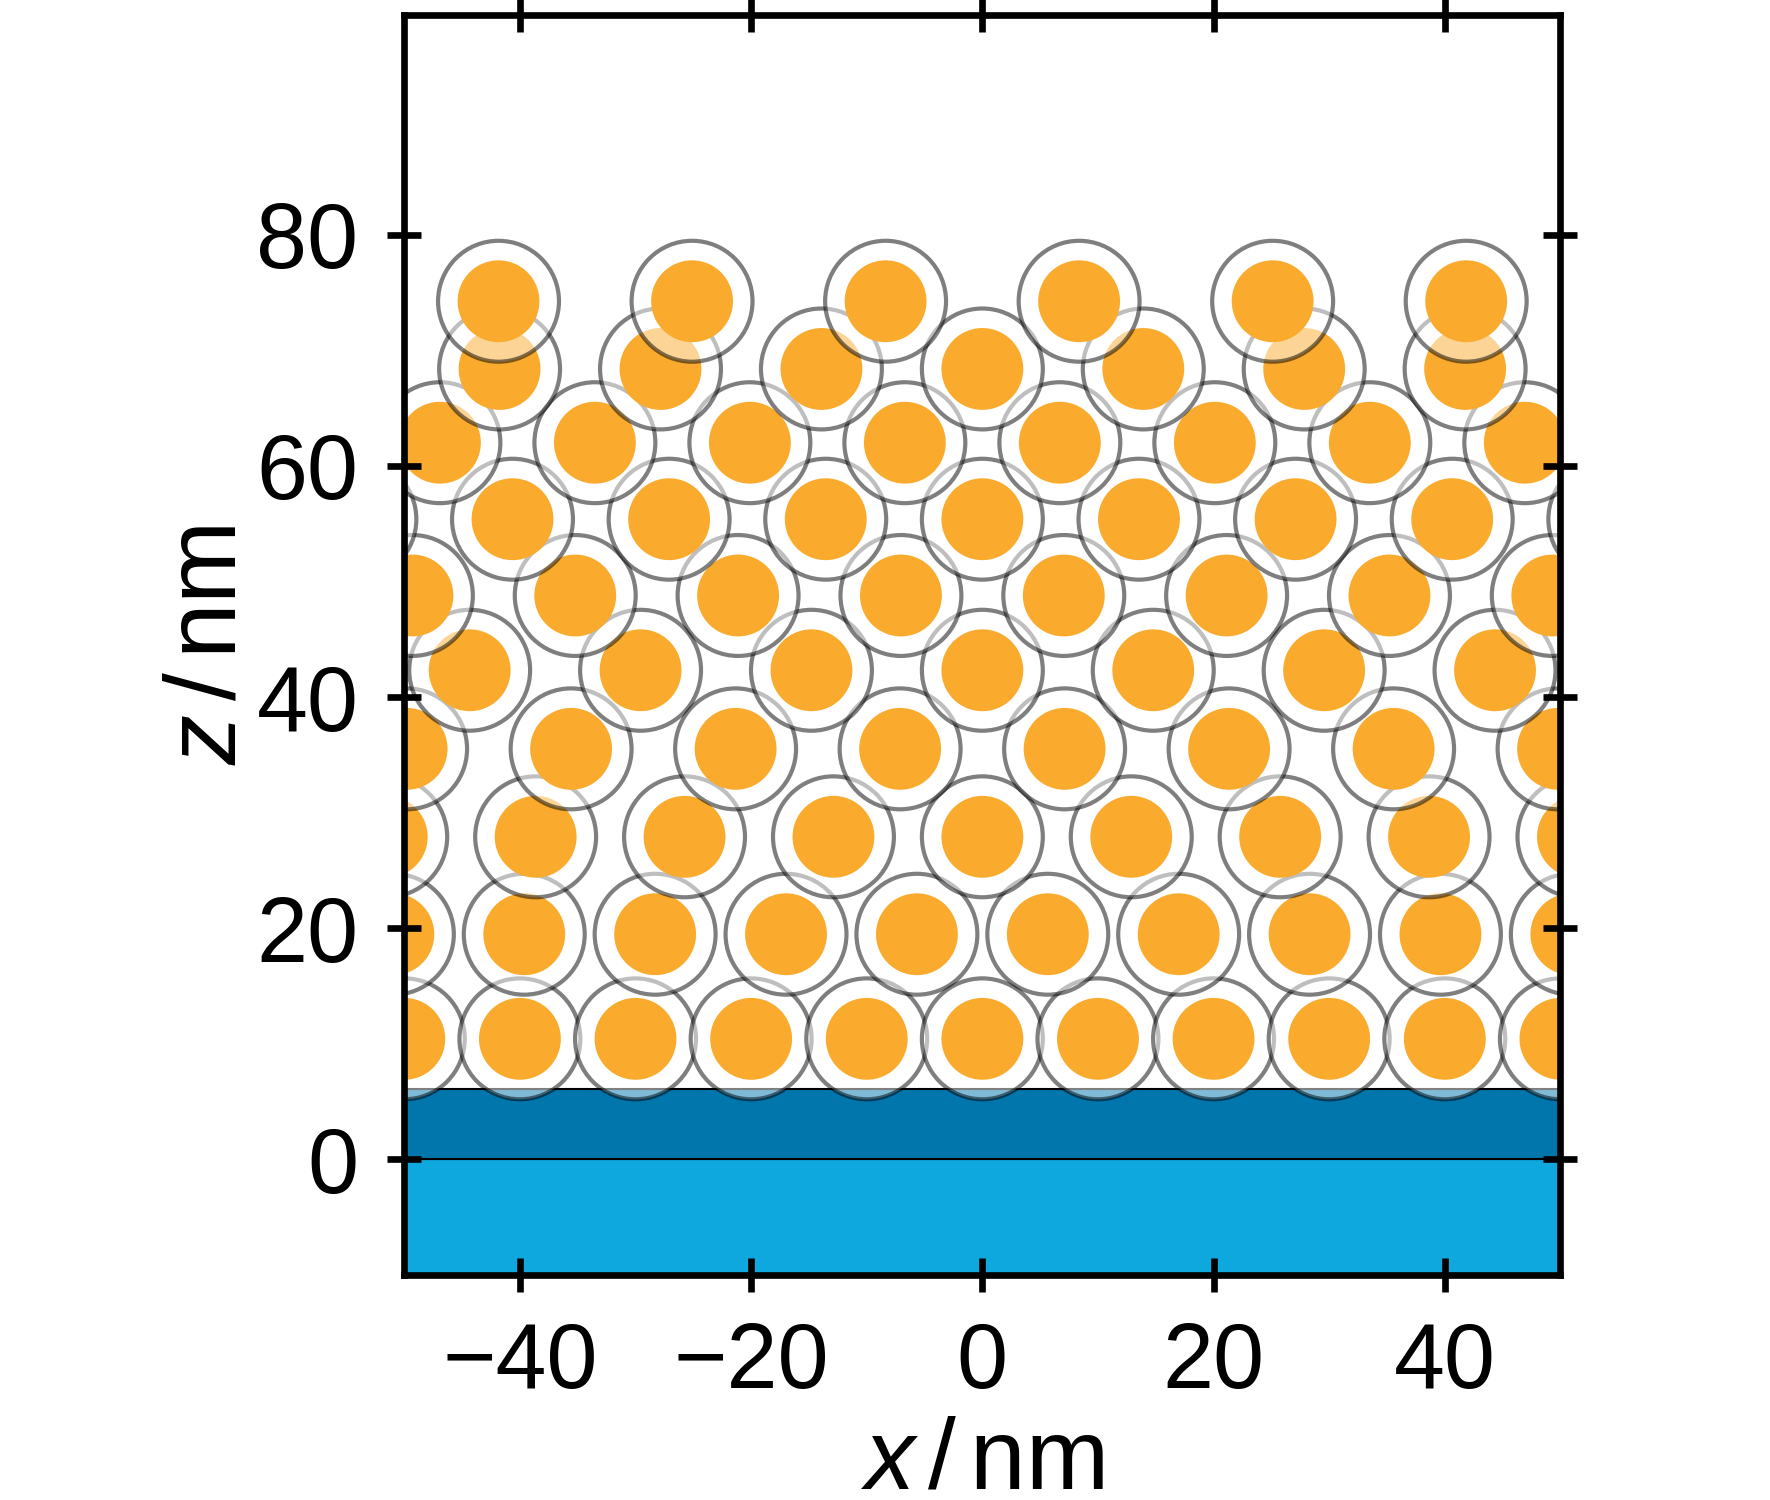
\includegraphics{looselyPackedNP_VerticalStructure_SC-IOS-7_PNRDepiction}
    \caption{\label{fig:looselyPackedNP:layer:xrrDepiction}Depiction generated from the fitted parameters in \reftab{tab:looselyPackedNP:nanoparticle:xrr} showing the average particle distance and layer packing.}
  \end{figure}

\end{document}